\documentclass{article}
\usepackage[utf8]{inputenc}
\usepackage{amsmath}
\usepackage{amssymb} 
\usepackage{amsthm}
\usepackage{enumitem}
\usepackage[english]{babel}
\usepackage[textheight=10in]{geometry}
\usepackage{tikz}
\tikzset{
  treenode/.style = 	{shape=rectangle, rounded corners,
				draw, align=center,
				top color=white, bottom color=blue!30},
  no/.style = 	{treenode, bottom color=red!30},
  yes/.style = 	{treenode, bottom color=green!30},
  env/.style = 	{treenode, font=\ttfamily\normalsize},
}


\begin{document}
\begin{enumerate}

\item On the first round, we must consider all the attribute choices.  We thus have:
	\begin{align*}
		ENT(A, d) &= ENT(a, d) + ENT(\bar a, d) \\
			&= Pr(a) \big[-Pr(d|a) \cdot \text{\text{log}}_2(Pr(d|a)) 
					-Pr(d|a) \cdot \text{\text{log}}_2(Pr(d|a)) \big]\\
				& \indent + Pr(\bar a)  \big[-Pr(d|\bar a) \cdot \text{\text{log}}_2(Pr(d|\bar a)) 
					- Pr(d|\bar a) \cdot \text{\text{log}}_2(Pr(d|\bar a)) \big] \\
			&= \frac {12} {23} 
					\left[ -\frac {3} {12} \text{\text{log}}_2\left(\frac{3}{12} \right) 
					- \frac{9}{12} \text{\text{log}}_2\left( \frac{9}{12} \right) \right]
				+ \frac {11} {23} 
					\left[ -\frac {7} {11} \text{\text{log}}_2 \left(\frac{7}{11} \right) 
					- \frac{4}{11} \text{\text{log}}_2 \left(\frac{4}{11} \right) \right]\\
			&\approx 0.876\\
		ENT(B, d) &= ENT(b, d) + ENT(\bar b, d) \\
			&= Pr(b) \big[-Pr(d|b) \cdot \text{\text{log}}_2(Pr(d|b)) 
					-Pr(d|b) \cdot \text{\text{log}}_2(Pr(d|b)) \big]\\
				& \indent + Pr(\bar b)  \big[-Pr(d|\bar b) \cdot \text{\text{log}}_2(Pr(d|\bar b)) 
					- Pr(d|\bar b) \cdot \text{\text{log}}_2(Pr(d|\bar b)) \big] \\
			&= \frac {9} {23} 
					\left[ -\frac {2} {9} \text{\text{log}}_2\left(\frac{2}{9} \right) 
					- \frac{7}{9} \text{\text{log}}_2\left( \frac{7}{9} \right) \right]
				+ \frac {14} {23} 
					\left[ -\frac {8} {14} \text{\text{log}}_2 \left(\frac{8}{14} \right) 
					- \frac{6}{14} \text{\text{log}}_2 \left(\frac{6}{14} \right) \right]\\
			&\approx 0.899\\
		ENT(C, d) &= ENT(c, d) + ENT(\bar c, d) \\
			&= Pr(c) \big[-Pr(d|c) \cdot \text{\text{log}}_2(Pr(d|c)) 
					-Pr(d|c) \cdot \text{\text{log}}_2(Pr(d|c)) \big]\\
				& \indent + Pr(\bar c)  \big[-Pr(d|\bar c) \cdot \text{\text{log}}_2(Pr(d|\bar c)) 
					- Pr(d|\bar c) \cdot \text{\text{log}}_2(Pr(d|\bar c)) \big] \\
			&= \frac {16} {23} 
					\left[ -\frac {6} {16} \text{\text{log}}_2\left(\frac{6}{16} \right) 
					- \frac{10}{16} \text{\text{log}}_2\left( \frac{10}{16} \right) \right]
				+ \frac {7} {23} 
					\left[ -\frac {4} {7} \text{\text{log}}_2 \left(\frac{4}{7} \right) 
					- \frac{3}{7} \text{\text{log}}_2 \left(\frac{3}{7} \right) \right]\\
			&\approx 0.964
	\end{align*}
	Since splitting on A results in the lowest entropy and thus greatest information gain, 
		we split on that first.  
	This results in \[ 
			\left \{ \begin{array} {lr}
				\{+ x_5, +x_7, - x_6, -x_8\}, & \text{for } A=F\\
			 	\{+ x_1, +x_2, - x_3, -x_4\}, & \text{for } A=T
			\end{array}\right\}
		\]
	At this point we have completed our search, since $ENT(C | \bar a) = ENT(B | a) = 0$.\\
	Therefore, our resulting tree is:
	\begin{center}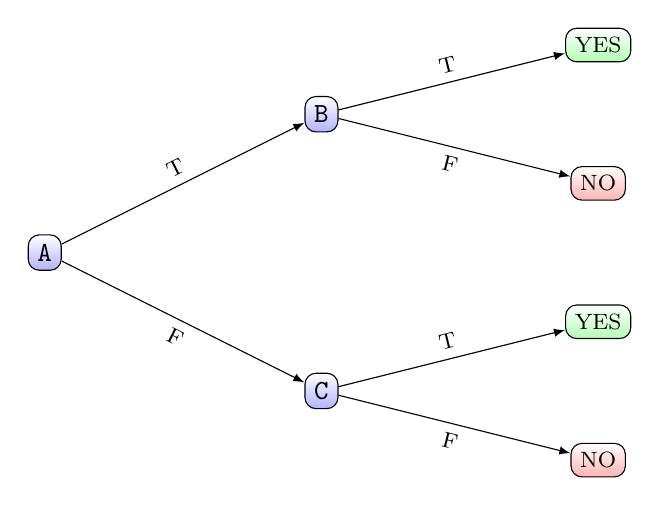
\begin{tikzpicture}
	[
		grow                    = right,
		sibling distance        = 5em,
		level distance          = 10em,
		edge from parent/.style = {draw, -latex},
		every node/.style       = {font=\footnotesize},
		sloped
	]
	\node [env] {A}
		child { node [env] {C}
			child { node [no] {NO}
				edge from parent node [below, align=center] {F}}
			child { node [yes] {YES}
				edge from parent node [above, align=center] {T}}
			edge from parent node [below] {F} }
		child [ missing ]
		child { node [env] {B}
			child { node [no] {NO}
				edge from parent node [below, align=center] {F}}
			child { node [yes] {YES}
				edge from parent node [above, align=center] {T}}
			edge from parent node [above] {T} };
	\end{tikzpicture} \end{center}
\clearpage
\item We assume that all nodes utilize the step function with threshold t as labeled on the node.\\
	These are therefore of the form \begin{equation*}
		g(I) =  
			\left \{ \begin{array} {lr}
				1, & \text{for } I \geq t\\
				0, & \text{for } I < t\\
			\end{array}\right\}
		\end{equation*}
	Numbers appearing directly above or below an edge are weights.
	Thus our network is:
	 \begin{center}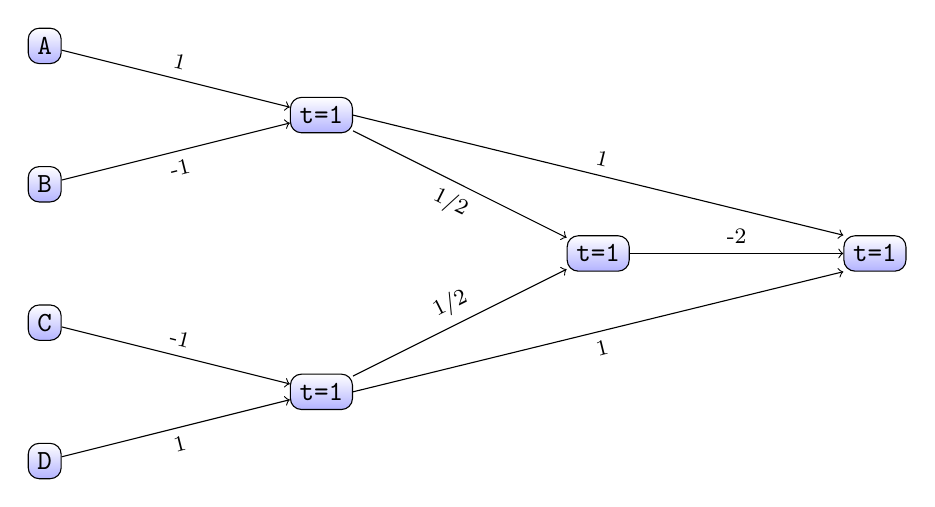
\begin{tikzpicture}
	[
		grow                    = left,
		sibling distance        = 5em,
		level distance          = 10em,
		edge from parent/.style = {<-, draw},
		every node/.style       = {font=\footnotesize},
		sloped
	]
	\node [env] (rt) {t=1}
		child {node [env] {t=1}
			child {node [env] (AND1){t=1}
				child {node [env] {A} 
					edge from parent node [above, align=center] {1}
				}
				child {node [env] {B} 
					edge from parent node [below, align=center] {-1}
				}
			edge from parent node [below, align=center] {1/2}
			}
			child [ missing ]
			child {node [env] (AND2){t=1}
				child {node [env] {C} 
					edge from parent node [above, align=center] {-1}
				}
				child {node [env] {D} 
					edge from parent node [below, align=center] {1}
				}
			edge from parent node [above, align=center] {1/2}
			}
			edge from parent node [above, align=center] {-2}
		};
	% generation-hopping
	\draw [->] (AND1.east) -- node  [above, midway] {1} (rt.north west);
	\draw [->] (AND2.east) -- node  [below, midway] {1} (rt.south west);
	\end{tikzpicture} \end{center}
\end{enumerate}
\end{document}